\section{Validazione e Collaudo}
\textit{Dal 2021-04-09 al 2021-05-03}


\begin{figure}[H]
	\centering
	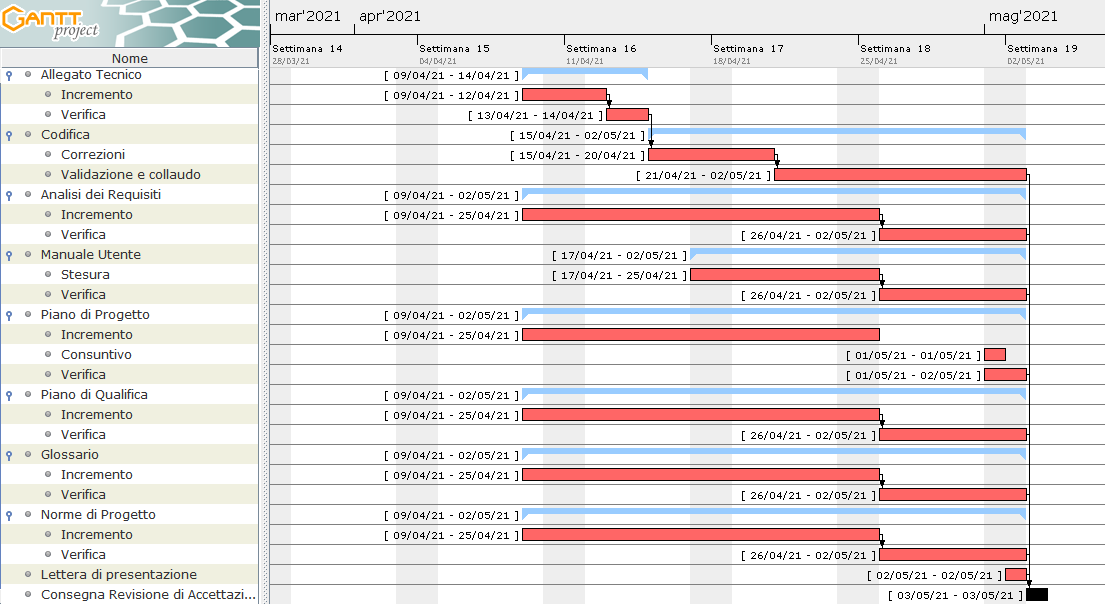
\includegraphics[scale=0.51]{res/images/06_gantt_validazione}
	\caption{Diagramma di gantt\textsubscript{G} relativo alla fase\textsubscript{G} di Validazione e Collaudo}
\end{figure}


\subsection{Periodo 1}

\subsubsection{Pianificazione preventiva}

\paragraph{Attività}

\planningTable{
	Incremento Analisi dei Requisiti & L'avanzamento nello sviluppo del prodotto chiarirà alcuni aspetti che nella fase\textsubscript{G} di Analisi risultavano oscuri, e potrebbe evidenziare delle criticità non inizialmente considerate. Se necessario, viene raffinata l'\textsc{Analisi dei Requisiti} &  & Verificatore
\tabularnewline 
Incremento Piano di Progetto & Il \textsc{Piano di Progetto} viene migliorato fornendo maggior dettaglio, oltre che integrato con il consuntivo del periodo trascorso &  & Responsabile
\tabularnewline 
Incremento Glossario & Viene integrato con nuovi termini &  & Responsabile
\tabularnewline 
Incremento Piano di Qualifica & Il cruscotto viene aggiornato con i dati rilevati sul periodo trascorso &  & Responsabile
\tabularnewline 
\caption{Pianificazione preventiva - Validazione e Collaudo - Periodo 1}
}

\paragraph{Preventivo}


\subsubsection{Pianificazione di periodo}

% gantt\textsubscript{G} @nicolò

\paragraph{Attività}

\paragraph{Preventivo orario ed economico}



\subsubsection{Riscontro di fine periodo}


\paragraph{Consuntivo orario ed economico}


\paragraph{Preventivo a finire}





\subsection{Periodo 2}

\subsubsection{Pianificazione preventiva}

\paragraph{Attività}

\planningTable{
	Validazione e Collaudo & vengono eseguiti ulteriori test per consolidare e garantire la qualità del prodotto. Il \textsc{Piano di Qualifica} è il documento di riferimento per quest'attività. &  & Verificatore
\tabularnewline 
Manuale Utente & Il \textsc{Manuale Utente} specifica le modalità d'uso del software agli utenti utilizzatori &  & Progettista
\tabularnewline 
Documentazione delle API & Come richiesto dal proponente, la documentazione conterrà le API di comunicazione tra server e unità &  & Progettista
\tabularnewline 
Lista dei bug & Come richiesto dal proponente, la documentazione conterrà i bug riscontrati durante lo sviluppo del software &  & Progettista
\tabularnewline 
\caption{Pianificazione preventiva - Validazione e Collaudo - Periodo 2}
}

\paragraph{Preventivo}

\subsubsection{Pianificazione di periodo}

% gantt\textsubscript{G} @nicolò

\paragraph{Attività}

\paragraph{Preventivo orario ed economico}



\subsubsection{Riscontro di fine periodo}


\paragraph{Consuntivo orario ed economico}


\paragraph{Preventivo a finire}






\subsection{Periodo 3}

\subsubsection{Pianificazione preventiva}

\paragraph{Attività}

\planningTable{
	Preparazione alla presentazione & Viene preparato il materiale necessario alla presentazione & 3 & Amministratore
\tabularnewline 
\caption{Pianificazione preventiva - Validazione e Collaudo - Periodo 3}
}

\paragraph{Preventivo}

\subsubsection{Pianificazione di periodo}


% gantt\textsubscript{G} @nicolò


\paragraph{Attività}

\paragraph{Preventivo orario ed economico}



\subsubsection{Riscontro di fine periodo}


\paragraph{Consuntivo orario ed economico}


\paragraph{Preventivo a finire}
